\chapter{Random Variables and Expected Value}

\section{What Is a Random Variable?}\index{random variable}
A \index{random variable}\newterm{random variable} assigns a number to each
outcome of a random experiment. Rolling a die gives an outcome, and the random
variable $X$ is the number that shows. Flipping a coin twice has four outcomes, and
the random variable $X$ can be the number of heads.

A \newterm{discrete} random variable takes a countable set of values. Its
\index{probability mass function}\newterm{probability mass function} (PMF) lists
each value and its probability. For two coin flips:

\begin{center}
\begin{tabular}{|c|c|}
\hline
$x$ (number of heads) & $P(X = x)$ \\
\hline
0 & $\frac{1}{4}$ \\
\hline
1 & $\frac{1}{2}$ \\
\hline
2 & $\frac{1}{4}$ \\
\hline
\end{tabular}
\end{center}

The probabilities must add up to 1.

\section{Expected Value}\index{expected value}
The \newterm{expected value} of $X$ is the average value we would get over many
repetitions. For a discrete random variable,
$$E[X] = \sum_x x \cdot P(X = x)$$
For the coin example, $E[X] = 0 \cdot \frac{1}{4} + 1 \cdot \frac{1}{2} + 2 \cdot
\frac{1}{4} = 1$.

The expected value does not have to be a value the variable can take. A fair
die has $E[X] = \frac{7}{2}$, even though no roll gives 3.5.

\section{Variance and Standard Deviation}\index{variance!random variable}
The \newterm{variance} measures how far $X$ typically is from its mean $\mu = E[X]$:
$$\operatorname{Var}(X) = E[(X - \mu)^2] = E[X^2] - \mu^2$$
The standard deviation is $\sigma = \sqrt{\operatorname{Var}(X)}$.

For a fair die, $E[X^2] = \frac{1 + 4 + 9 + 16 + 25 + 36}{6} = \frac{91}{6}$, so
$$\operatorname{Var}(X) = \frac{91}{6} - \left(\frac{7}{2}\right)^2 = \frac{35}{12}$$

\section{Linearity of Expectation}\index{linearity of expectation}
Expected value is linear. For constants $a$ and $b$:
$$E[aX + b] = aE[X] + b \qquad \operatorname{Var}(aX + b) = a^2\operatorname{Var}(X)$$
Adding a constant shifts the mean but does not change the spread.

If $X$ and $Y$ are independent, their variances add:
$\operatorname{Var}(X + Y) = \operatorname{Var}(X) + \operatorname{Var}(Y)$.
For two dice, the sum $S$ has $E[S] = 7$ and $\operatorname{Var}(S) = 2 \cdot \frac{35}{12} = \frac{35}{6}$.

\section{A Game Example}
A game costs \$10 to enter. You win \$30 with probability $\frac{1}{4}$ and win
nothing otherwise. Let $W$ be your net winnings. Then $W = 30 - 10 = 20$ with
probability $\frac{1}{4}$ and $W = -10$ with probability $\frac{3}{4}$. So
$$E[W] = 20 \cdot \frac{1}{4} + (-10) \cdot \frac{3}{4} = -2.5$$
On average, you lose \$2.50 per game.

\begin{Exercise}[label=rv1, title=Expected value of a die]
Let $X$ be the number on a fair six-sided die. Find $E[2X + 1]$.
\end{Exercise}
\begin{Answer}[ref=rv1]
$E[2X + 1] = 2 \cdot \frac{7}{2} + 1 = 8$.
\end{Answer}

\begin{Exercise}[label=rv2, title=Variance after scaling]
Using the die from the previous exercise, find $\operatorname{Var}(2X + 1)$.
\end{Exercise}
\begin{Answer}[ref=rv2]
$\operatorname{Var}(2X + 1) = 4 \cdot \frac{35}{12} = \frac{35}{3}$.
\end{Answer}

\begin{Exercise}[label=rv3, title=Two coin flips]
Use the PMF table above to check that $E[X] = 1$ and $\operatorname{Var}(X) = \frac{1}{2}$.
\end{Exercise}
\begin{Answer}[ref=rv3]
$E[X^2] = 0 + \frac{1}{2} + 1 = \frac{3}{2}$, so $\operatorname{Var}(X) = \frac{3}{2} - 1 = \frac{1}{2}$.
\end{Answer}

\begin{Exercise}[label=rv4, title=Is the game worth playing?]
A game costs \$5 to enter. You win \$20 with probability $\frac{1}{5}$ and nothing
otherwise. What is the expected net winnings? Should you play?
\end{Exercise}
\begin{Answer}[ref=rv4]
The net winnings are $15$ with probability $\frac{1}{5}$ and $-5$ with probability
$\frac{4}{5}$. The expected value is $3 - 4 = -1$. The expected loss is \$1 per
game, so the game is not worth playing.
\end{Answer}

\section{Expected Value/Mean}
How can we find the average (mean) of a variable with a given probability 
distribution function? Consider the example of transaction processing times. 
If we knew the total time spent processing transactions and the total number 
of customers, then the mean processing time would be the total processing time 
divided by the total number of customers. 

Suppose we have a PDF that describes processing time for electronic 
transactions, $f(t)$, where $t$ is processing time and $f(t)$ is the 
probability that an individual transaction takes a particular amount of time, 
$t$. Electronic transactions are fast, and we can assume no transaction takes longer than 250 milliseconds, so we restrict the domain of $f(t)$ to $0 \leq t \leq 250$. We can divide the PDF into intervals of width $\Delta t$ (see figure 
\ref{fig:mean}). 

\begin{figure}[H]
    \centering
    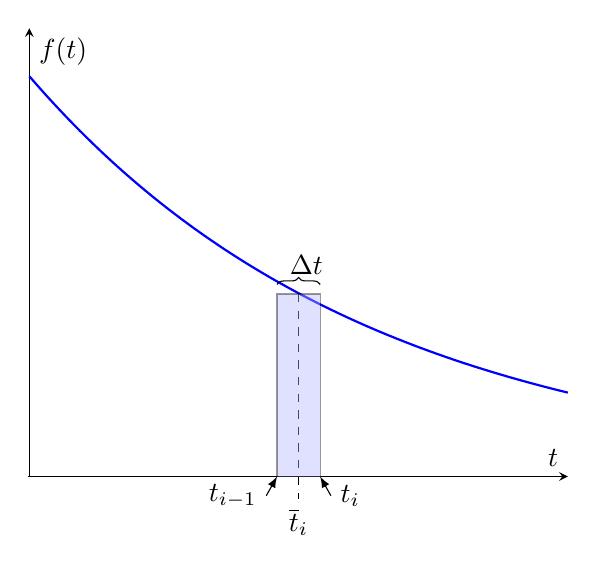
\begin{tikzpicture}
	\begin{axis}[xmin = -0.5, xmax = 250, ymin = 0, ymax = 0.007, axis lines = 
	center, xlabel = $t$, ylabel = $f(t)$, ticks = none, clip = false]
		\addplot[blue, thick, domain = 0:250, samples = 300] {(1/160)*e^(-1*x/160)};
        \draw[black, dashed] (125, 0.00285) -- (125, -0.00035) node[below] {
        $\overline{t}_i$};
        \draw[black, fill = blue!30, opacity = 0.4] (115, 0) rectangle 
        (135, 0.00285);
        \draw[latex-] (115, 0) -- (110, -0.0003) node[left] {$t_{i-1}$};
        \draw[latex-] (135, 0) -- (140, -0.0003) node[right] {$t_i$};
        \draw[decorate, decoration = brace] (115, 0.003) -- (135, 0.003) 
        node[above, xshift = -5] {$\Delta t$};
		\end{axis}
	\end{tikzpicture}
    \label{fig:mean}
    \caption{The probability that an individual transaction takes between 
    $t_{i-1}$ and $t_i$ seconds is approximated by the shaded area}
\end{figure}

If a total of $N$ transactions are processed, then the number of transactions 
that take between $t_{i-1}$ and $t_i$ is the probability of a transaction 
taking between $t_{i-1}$ and $t_i$ times $N$. That probability is approximately $f(\overline{t}_i) \Delta t$, and so the number of transactions taking between 
$t_{i-1}$ and $t_i$ is $Nf(\overline{t}_i) \Delta t$. Each of these 
transactions took approximately $\overline{t}_i$, and therefore the total 
processing time for these transactions is the number of transactions multiplied
by the processing time:
$$\overline{t}_i \left[ N f(\overline{t}_i) \Delta t \right]$$

To find the total processing time for all transactions, we would add up the 
total processing time for each interval:
$$\sum_{i = 1}^n N \overline{t}_i f(\overline{t}_i) \Delta t$$

And to find the average or mean processing time, we would divide this sum by 
the total number of customers, $N$:
$$\text{mean processing time} = \sum_{i = 1}^n \overline{t}_i f(\overline{
t}_i) \Delta t$$

Taking the limit as $n \to \infty$, the sum becomes an integral:
$$\text{mean processing time} = \int_0^{250} t \cdot f(t)\,dt$$

Recall that we use $\mu$ to represent the mean. Therefore, for a general PDF, 
$f(x)$, the mean is given by:
$$\mu = \int_{-\infty}^{\infty} x \cdot f(x)\,dx$$

\textbf{Example}: Find the mean value of the general exponential PDF, 
$$f(x) = 
\begin{cases}
0,&\text{if }x < 0\\
ce^{-cx},&\text{if }x \geq 0
\end{cases}$$

\textbf{Solution}: Applying the definition of the mean:
$$\mu = \int_{-\infty}^{\infty} xf(x)\,dx = \int_0^{\infty} xce^{-cx}\,dx$$
$$= -xe^{-cx}|_{x = 0}^{x = \infty} - \int_0^{\infty} -e^{-cx}\,dx$$
$$= 0 + \left[-\frac{1}{c}e^{-cx} \right]_{x = 0}^{x = \infty} = \frac{1}{c}$$

And since $\mu = 1/c$, we can re-write the general exponential PDF in terms of 
the mean:
$$f(x) = 
\begin{cases}
0,&\text{if }x < 0\\
\mu^{-1}e^{-x/\mu},&\text{if }x \geq 0
\end{cases}$$

\begin{Exercise}[title = {Onset of Symptoms}, label = symptoms]
Researchers find that the time between infection by the COVID virus and the 
onset of symptoms can be described by the PDF:
$$f(t) = 
\begin{cases}
\frac{1}{595} te^{-0.04t},&\text{if }0 \leq t \leq 120\\
0,&\text{otherwise}
\end{cases}$$

What is the mean time between infection and the onset of symptoms?
\vspace{50mm}
\end{Exercise}

\begin{Answer}[ref = symptoms]
$$\mu = \int_{-\infty}^{\infty} tf(t)\,dt = \frac{1}{595} \int_{0}^{120} t^2 e^{-0.04t}\,dt$$

Integrate by parts twice, or use the antiderivative
$$\int t^2 e^{-at}\,dt = -e^{-at}\left(\frac{t^2}{a} + \frac{2t}{a^2} + \frac{2}{a^3}\right)$$
with $a = 0.04$. Evaluating from $0$ to $120$ gives
$$\mu = \frac{1}{595}\left(31250 - 541250\,e^{-4.8}\right) = \frac{6250 - 108250\,e^{-4.8}}{119} \approx 45.04$$

Therefore, the mean time until the onset of symptoms is approximately 45 hours.
\end{Answer}

\section{Expected Values for Two Variables}
Recall that for one variable, $X$, the expected value of $X$ (its mean) is:
$$\mu = \int_{- \infty}^{\infty} xf(x)\,dx$$

Where $f(x)$ is the probability density function for $X$. Expanding this to two
independent random variables, $X$ and $Y$, we find the expected values for each
variable are:
$$\mu_x = \iint_{\mathbb{R}^2} xf(x, y)\,dA$$
$$\mu_y = \iint_{\mathbb{R}^2} yf(x, y)\,dA$$

\textbf{Example}: $X$ and $Y$ are random variables with joint density function:
$$f(x, y) = 
\begin{cases}
0.1e^{-(0.2x + 0.5y)},&\text{if } x \geq 0,\text{ }y \geq 0\\
0,&\text{otherwise}
\end{cases}$$

What are the expected values of $X$ and $Y$?

\textbf{Solution}: The expected value of $X$ is:
$$\mu_x = \int_0^{\infty} \int_0^{\infty} x(0.1)e^{-(0.2x + 0.5y)}\,dy\,dx$$
$$= \frac{1}{10} \int_0^{\infty} x \left(-2 \right) e^{-(0.2x + 0.5y)}|_{y = 0}
^{y = \infty}\,dx = -\frac{1}{5} \int_0^{\infty} (x)e^{-0.2x} \left[ e^{-0.5y} 
\right]_{y = 0}^{y = \infty}\,dx$$
$$= -\frac{1}{5} \int_0^{\infty} xe^{-0.2x} \left[ e^{-\infty} - e^0 \right]
\,dx = -\frac{1}{5} \int_0^{\infty} xe^{-0.2x} \left[0 - 1 \right]\,dx $$
$$= \frac{1}{5} \int_0^{\infty} xe^{-0.2x}\,dx$$

Applying integration by parts, 
$$\mu_x = \frac{1}{5} \left[ -5xe^{-0.2x}|_{x = 0}^{x = \infty} - \int_0^{
\infty} (-5)e^{-0.2x}\,dx \right]$$
$$= \left[-xe^{-0.2x} \right]_{x = 0}^{x = \infty} + \int_0^{\infty} e^{-0.2x}
\,dx  = -5e^{-0.2x}|_{x = 0}^{x = \infty}$$
$$= -5 \left(e^{-\infty} - e^0 \right) = -5 \left(0 - 1 \right) = 5$$

And the expected value of $Y$ is:
$$\mu_y = \int_0^{\infty} \int_0^{\infty} y(0.1)e^{-(0.2x + 0.5y)}\,dx\,dy$$
$$= \frac{1}{10} \int_0^{\infty} (y)e^{-0.5y} \int_0^{\infty} \left(e^{-0.2x} 
\right)\,dx\,dy = \frac{1}{10} \int_0^{\infty} (y)e^{-0.5y} \left[ -5e^{-0.2x} 
\right]_{x = 0}^{x = \infty}\,dy$$
$$= \frac{1}{10} \int_0^{\infty} (y)e^{-0.5y} \left(0 + 5 \right)\,dy = \frac{
1}{2} \int_0^{\infty} ye^{-0.5y}\,dy$$

Applying integration by parts:
$$\mu_y = \frac{1}{2} \left[(-2)ye^{-0.5y}|_{y = 0}^{y = \infty} - \int_0^{
\infty} (-2)e^{-0.5y}\,dy \right]$$
$$= \left[-ye^{-0.5y} \right]_{y = 0}^{y = \infty} + (-2)e^{-0.5y}|_{y = 0}^{y 
= \infty} = (-2) \left( e^{-\infty} - e^0 \right) = -2(0 - 1) = 2$$

Therefore, the expected value of $X$ is 5 and of $Y$ is 2. 

\begin{Exercise}[title = {Expected Values}, label = expect]
The joint density function for a pair of random variables, $X$ and $Y$ is
$$f(x, y) = 
\begin{cases}
	\frac{1}{4} y (1 + 2x),& \text{if } 0 \leq x \leq 1\text{, }0 \leq y \leq 2\\
	0,&\text{ otherwise}
\end{cases}$$
What are the expected values of $X$ and $Y$?
\vspace{75mm}
\end{Exercise}

\begin{Answer}[ref = expect]
Finding the expected value of $X$:
$$\mu_x = \int_0^1 \int_0^2 \frac{1}{4}xy \left(1 + 2x \right)\,dy\,dx = 
\frac{1}{4} \int_0^1 x \left( 1 + 2x \right) \int_0^2 y\,dy\,dx$$
$$= \frac{1}{4} \int_0^1 x \left( 1 + 2x \right) \left[ \frac{1}{2} y^2 \right]_
{y = 0}^{y = 2}\,dx = \frac{1}{4} \int_0^1 x \left(1 + 2x \right) (2)\,dx$$
$$= \frac{1}{2} \int_0^1 x + 2x^2\,dx = \frac{1}{2} \left[ \frac{1}{2}x^2 + 
\frac{2}{3}x^3 \right]_{x = 0}^{x = 1}$$
$$= \frac{1}{2} \left( \frac{1}{2} + \frac{2}{3} \right) = \frac{1}{2} \left( 
\frac{7}{6} \right) = \frac{7}{12}$$

And finding the expected value of $Y$:
$$\mu_y = \int_0^2 \int_0^1 \frac{1}{4}y^2 \left(1 + 2x \right)\,dx\,dy = 
\frac{1}{4} \int_0^2 y^2 \int_0^1 \left( 1 + 2x \right)\,dx\,dy$$
$$= \frac{1}{4} \int_0^2 y^2 \left[x + x^2 \right]_{x = 0}^{x = 1}\,dy = 
\frac{1}{4} \int_0^2 y^2 (2)\,dy$$
$$= \frac{1}{2} \int_0^2 y^2\,dy = \frac{1}{2} \left[ \frac{1}{3}y^3 \right]_{
y = 0}^{y = 2} = \frac{1}{2} \left( \frac{1}{3} \right) (8) = \frac{4}{3}$$
\end{Answer}
